%% LyX 2.3.4.2 created this file.  For more info, see http://www.lyx.org/.
%% Do not edit unless you really know what you are doing.
\documentclass[11pt,oneside,czech,american]{book}
\usepackage[T1]{fontenc}
\usepackage[utf8]{inputenc}
\usepackage[a4paper]{geometry}
\geometry{verbose,tmargin=4cm,bmargin=3cm,lmargin=3cm,rmargin=2cm,headheight=0.8cm,headsep=1cm,footskip=0.5cm}
\pagestyle{headings}
\setcounter{secnumdepth}{3}
\usepackage{url}
\usepackage{amsmath}
\usepackage{amsthm}
\usepackage{amssymb}
\usepackage{graphicx}
\usepackage{setspace}
\usepackage{subfig}
\usepackage{tikz}

\makeatletter
%%%%%%%%%%%%%%%%%%%%%%%%%%%%%% Textclass specific LaTeX commands.
\newenvironment{lyxlist}[1]
	{\begin{list}{}
		{\settowidth{\labelwidth}{#1}
		 \setlength{\leftmargin}{\labelwidth}
		 \addtolength{\leftmargin}{\labelsep}
		 \renewcommand{\makelabel}[1]{##1\hfil}}}
	{\end{list}}

%%%%%%%%%%%%%%%%%%%%%%%%%%%%%% User specified LaTeX commands.
%% Font setup: please leave the LyX font settings all set to 'default'
%% if you want to use any of these packages:

%% Use Times New Roman font for text and Belleek font for math
%% Please make sure that the 'esint' package is turned off in the
%% 'Math options' page.
\usepackage[varg]{txfonts}

%% Use Utopia text with Fourier-GUTenberg math
%\usepackage{fourier}

%% Bitstream Charter text with Math Design math
%\usepackage[charter]{mathdesign}

%%---------------------------------------------------------------------

%% Make the multiline figure/table captions indent so that the second
%% line "hangs" right below the first one.
%\usepackage[format=hang]{caption}

%% Indent even the first paragraph in each section
\usepackage{indentfirst}

%%---------------------------------------------------------------------

%% Disable page numbers in the TOC. LOF, LOT (TOC automatically
%% adds \thispagestyle{chapter} if not overriden
%\addtocontents{toc}{\protect\thispagestyle{empty}}
%\addtocontents{lof}{\protect\thispagestyle{empty}}
%\addtocontents{lot}{\protect\thispagestyle{empty}}

%% Shifts the top line of the TOC (not the title) 1cm upwards 
%% so that the whole TOC fits on 1 page. Additional page size
%% adjustment is performed at the point where the TOC
%% is inserted.
%\addtocontents{toc}{\protect\vspace{-1cm}}

%%---------------------------------------------------------------------

% completely avoid orphans (first lines of a new paragraph on the bottom of a page)
\clubpenalty=9500

% completely avoid widows (last lines of paragraph on a new page)
\widowpenalty=9500

% disable hyphenation of acronyms
\hyphenation{CDFA HARDI HiPPIES IKEM InterTrack MEGIDDO MIMD MPFA DICOM ASCLEPIOS MedInria}

%%---------------------------------------------------------------------

%% Print out all vectors in bold type instead of printing an arrow above them
\renewcommand{\vec}[1]{\boldsymbol{#1}}
\newcommand{\E}{\mathbb{E}} 
% Replace standard \cite by the parenthetical variant \citep
%\renewcommand{\cite}{\citep}

\makeatother

\usepackage{babel}
\begin{document}
\def\documentdate{June 1, 2021}

%%\def\documentdate{\today}

\pagestyle{empty}
{\centering

\noindent %
\begin{minipage}[c]{3cm}%
\noindent \begin{center}
\includegraphics[width=3cm,height=3cm,keepaspectratio]{Images/TITLE/cvut}
\par\end{center}%
\end{minipage}%
\begin{minipage}[c]{0.6\linewidth}%
\begin{center}
\textsc{\large{}Czech Technical University in Prague}{\large{}}\\
{\large{}Faculty of Nuclear Sciences and Physical Engineering}
\par\end{center}%
\end{minipage}%
\begin{minipage}[c]{3cm}%
\noindent \begin{center}
\includegraphics[width=3cm,height=3cm,keepaspectratio]{Images/TITLE/fjfi}
\par\end{center}%
\end{minipage}

\vspace{3cm}

\textbf{\huge{}Generative and discriminative models for set data}{\huge\par}

\vspace{1cm}

\selectlanguage{czech}%
\textbf{\huge{}Generativní a diskriminativní modely pro množinová data}{\huge\par}

\selectlanguage{american}%
\vspace{2cm}

{\large{}Research Project}{\large\par}

}

\vfill{}

\begin{lyxlist}{MMMMMMMMM}
\begin{singlespace}
\item [{Author:}] \textbf{Bc. Jakub Bureš}
\item [{Supervisor:}] \textbf{doc. Ing. Václav Šmídl, Ph.D.}
\end{singlespace}
\item [{Language~advisor:}] \textbf{Mgr. }
\begin{singlespace}
\item [{Academic~year:}] 2020/2021
\end{singlespace}
\end{lyxlist}

~\newpage{}

\noindent \emph{\Large{}Acknowledgment:}{\Large\par}

\noindent I would like to thank ............................................
for (his/her expert guidance) and express my gratitude to ..........................................
for (his/her language assistance).

\vfill

\noindent \emph{\Large{}Author's declaration:}{\Large\par}

\noindent I declare that this Bachelor's Degree Project is entirely
my own work and I have listed all the used sources in the bibliography.

\bigskip{}

\noindent Prague, \documentdate\hfill{}Jméno Autora

\vspace{2cm}

\newpage{}

\selectlanguage{czech}%
\begin{onehalfspace}
\noindent \emph{Název práce:}

\noindent \textbf{Název práce}
\end{onehalfspace}

\bigskip{}

\noindent \emph{Autor:} Jméno Autora

\bigskip{}

\noindent \emph{Obor:} Celý název oboru (nikoliv zkratka)\bigskip{}

\noindent \emph{Zaměření:} Celý název zaměření (Pokud obor neobsahuje
zaměření, tuto řádku odstranit.)

\bigskip{}

\noindent \emph{Druh práce:} Bakalářská práce

\bigskip{}

\noindent \emph{Vedoucí práce:} prof. Ing. Jméno Školitele, DrSc.,
pracoviště školitele (název instituce, fakulty, katedry...)

\bigskip{}

\noindent \emph{Konzultant:} doc. RNDr. Jméno Konzultanta, CSc., pracoviště
konzultanta. Pouze pokud konzultant byl jmenován.

\bigskip{}

\noindent \emph{Abstrakt:} Abstrakt max. na 10 řádků. Abstrakt max.
na 10 řádků. Abstrakt max. na 10 řádků. Abstrakt max. na 10 řádků.
Abstrakt max. na 10 řádků. Abstrakt max. na 10 řádků. Abstrakt max.
na 10 řádků. Abstrakt max. na 10 řádků. Abstrakt max. na 10 řádků.
Abstrakt max. na 10 řádků. Abstrakt max. na 10 řádků. Abstrakt max.
na 10 řádků. Abstrakt max. na 10 řádků. Abstrakt max. na 10 řádků.
Abstrakt max. na 10 řádků. Abstrakt max. na 10 řádků. Abstrakt max.
na 10 řádků. Abstrakt max. na 10 řádků. Abstrakt max. na 10 řádků.
Abstrakt max. na 10 řádků. Abstrakt max. na 10 řádků. Abstrakt max.
na 10 řádků. Abstrakt max. na 10 řádků. Abstrakt max. na 10 řádků.
Abstrakt max. na 10 řádků. Abstrakt max. na 10 řádků. Abstrakt max.
na 10 řádků. Abstrakt max. na 10 řádků. Abstrakt max. na 10 řádků. 

\bigskip{}

\noindent \emph{Klíčová slova:} klíčová slova (nebo výrazy) seřazená
podle abecedy a oddělená čárkou

\selectlanguage{american}%
\vfill{}
~

\begin{onehalfspace}
\noindent \emph{Title:}

\noindent \textbf{Title of the Work}
\end{onehalfspace}

\bigskip{}

\noindent \emph{Author:} Author's Name

\bigskip{}

\noindent \emph{Abstract:} Max. 10 lines of English abstract text.
Max. 10 lines of English abstract text. Max. 10 lines of English abstract
text. Max. 10 lines of English abstract text. Max. 10 lines of English
abstract text. Max. 10 lines of English abstract text. Max. 10 lines
of English abstract text. Max. 10 lines of English abstract text.
Max. 10 lines of English abstract text. Max. 10 lines of English abstract
text. Max. 10 lines of English abstract text. Max. 10 lines of English
abstract text. Max. 10 lines of English abstract text. Max. 10 lines
of English abstract text. Max. 10 lines of English abstract text.
Max. 10 lines of English abstract text. Max. 10 lines of English abstract
text. Max. 10 lines of English abstract text. Max. 10 lines of English
abstract text. Max. 10 lines of English abstract text. Max. 10 lines
of English abstract text. Max. 10 lines of English abstract text.
Max. 10 lines of English abstract text. Max. 10 lines of English abstract
text. Max. 10 lines of English abstract text.

\bigskip{}

\noindent \emph{Key words:} keywords in alphabetical order separated
by commas

\newpage{}

\pagestyle{plain}

\tableofcontents{}

\newpage{}

\chapter*{Introduction}

\addcontentsline{toc}{chapter}{Introduction}

Paragraphs of the Introduction\ldots{}

\chapter{Multiple Instance Learning}
In standard machine learning problems each sample is represented by a fixed vector $\bold{x}$ of values, nevertheless in multiple instance learning (MIL) we deal with samples which are represented by a set of vectors. These vectors are called \textit{instances} and come from an instance space $\mathcal{X}$. Sets of these instances are called \textit{bags} and come from bag space $\mathcal{B} = \mathcal{P}_F\left(\mathcal{X}\right)$, where $\mathcal{P}_F\left(\mathcal{X}\right)$ denotes all finite subsets of $\mathcal{X}$. With this in mind, we can easily write down any bag $b$ as $b = \left\lbrace \bold{x} \in  \mathcal{X} \right\rbrace_{\bold{x} \in b}$. Each bag can be arbitrarily large or empty thus the size of bag $\vert b\vert \in \mathbb{N}_0$. There may exist intrinsic labeling of instances, but we are only interested in labeling at the bag levels. Bag labels come from a finite set $\mathcal{C}$ and what we want in MIL is learning a predictor in the form $f: \mathcal{B}\left(\mathcal{X}\right) \rightarrow \mathcal{C}$ which can also be rewritten in the form $f\left(\left\lbrace \bold{x}\right\rbrace_{\bold{x}\in b}\right)$. We consider supervised setting, in which each sample of the dataset is attributed a label. We can denote available data by $\mathcal{D} = \left\lbrace\left(b_i, y_i\right) \in \mathcal{B}\times\mathcal{C} \ | \ i \in \left\lbrace 1,2,\dots,\vert \mathcal{D} \vert \right\rbrace \right\rbrace$, where $\vert \mathcal{D} \vert$ denotes size of $\mathcal{D}$. 

\section{Cross-Validation}
Probably the simplest and most widely used method for estimating prediction error is \textit{cross-validation}. This method directly estimates the expected extra-sample error 
\begin{equation}
\mathrm{Err} = \E\left[L\left(Y, \hat{f}\left(X\right)\right)\right],
\end{equation}
the average generalization error when the method $\hat{f}\left(X\right)$ is applied to an independent test sample form the joint distribution of $X$ and $Y$- As mentioned earlier, we might hope that cross-validation estimates the conditional error, with the training set $\mathcal{T}$ held fixed. But cross-validation typically estimates well only the expected prediction error.

\subsection*{K-Fold Cross-Validation}
Ideally, if we had enough data, we would set aside a validation set and use
it to assess the performance of our prediction model. Since data are often
scarce, this is usually not possible. To finesse the problem, K-fold cross-validation
uses part of the available data to fit the model, and a different
part to test it. We split the data into $K$ roughly equal-sized parts; for
example, when $K = 5$, the scenario could look like this \\
\begin{center}
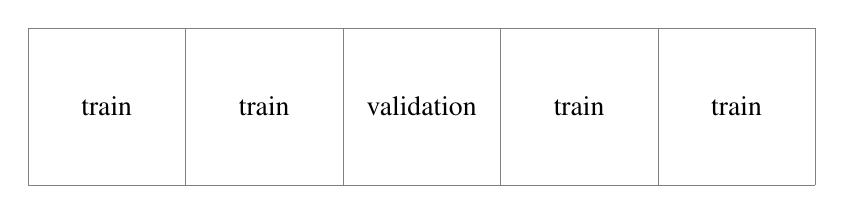
\begin{tikzpicture}
\draw[step=2cm,gray,very thin] (0,0) grid (10,2);
\draw (5,1) node{validation};
\draw (1,1) node{train};
\draw (3,1) node{train};
\draw (7,1) node{train};
\draw (9,1) node{train};
\end{tikzpicture}
\end{center}

For the $k$th part (third above), we fit the model to the other $K-1$ parts
of the data, and calculate the prediction error of the fitted model when
predicting the $k$th part of the data. We do this for $k = \left\lbrace 1,2,\dots,K\right\rbrace$ and
combine the $K$ estimates of prediction error.\\
Here are more details. Let $\kappa : \left\lbrace 1,\dots,N\right\rbrace\rightarrow  \left\lbrace 1,\dots,K\right\rbrace$ be an indexing
function that indicates the partition to which observation $i$ is allocated by
the randomization. Denote by $\hat{f}^{-k}\left(x\right)$ the fitted function, computed with
the $k$th part of the data removed. Then the cross-validation estimate of
prediction error is
\begin{equation}
\mathrm{CV}\left(\hat{f}\right) = \frac{1}{N}\sum_{i = 1}^{N}L\left(y_i , \hat{f}^{-\kappa\left(i\right)}\left(x_i\right)\right).
\end{equation}
Typical choices of K are 5 or 10 and even case $K = N$, which is known as \textit{leave-one-out} cross-validation.

\section{Experiment with mill datasets}
Suppose we have two classes 0 and 1 (known as binary classification), which means that bags are labeled either as 0 or 1. What happens, if we have many more bags, for example, labeled as class 1? This situation is very common in anomaly detection, where known anomalies are quite rare. \\
Let's assume train set is composed of 80\% bags labeled as 1 and 5\% bags labeled as 0, all randomly chosen. Test set is composed of 20\% bags labeled as 1 and 95\% labeled as 0, in other words it is complement of train set. Validation set is very similar to train set in terms of ratios, it contains 20\% bags labeled as 1 and 2\% bags labeled as 0. Train set is used to train our model, after that we evaluate loss function of the model with help of validation a test set, where number of dense layers is our hyperparameter. The purpose of this simulation is to find number of dense layer in which the loss is minimal and compare these 2 values. This experiment was performed 5 times then results were averaged, totally on 6 different datasets. 

 \begin{figure}[h]
\centering
\subfloat[]
{{\includegraphics[width=8.0cm]{Images/TITLE/Fox} }}%
\subfloat[]
{{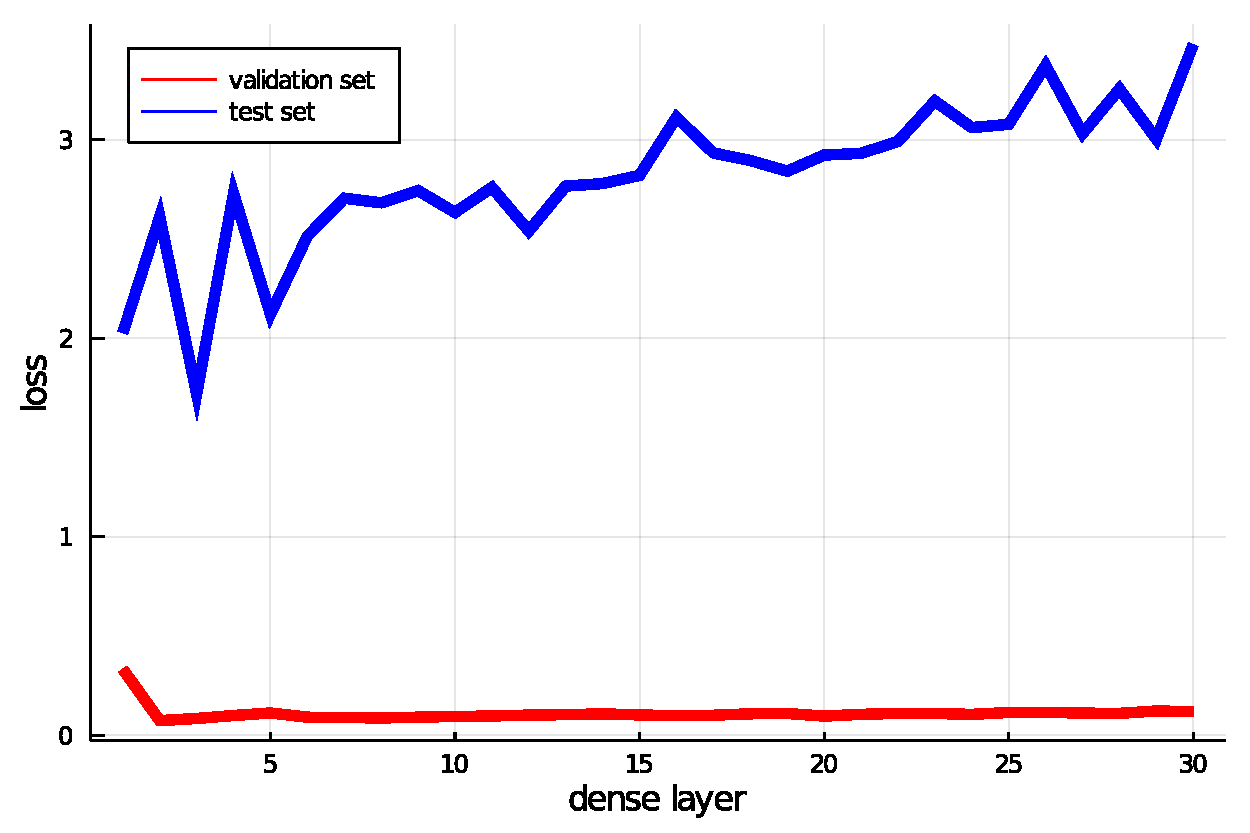
\includegraphics[width=8.0cm]{Images/TITLE/Elephant} }}%
\
 \subfloat[]
{{\includegraphics[width=8.0cm]{Images/TITLE/Tiger} }}%,
\subfloat[]
{{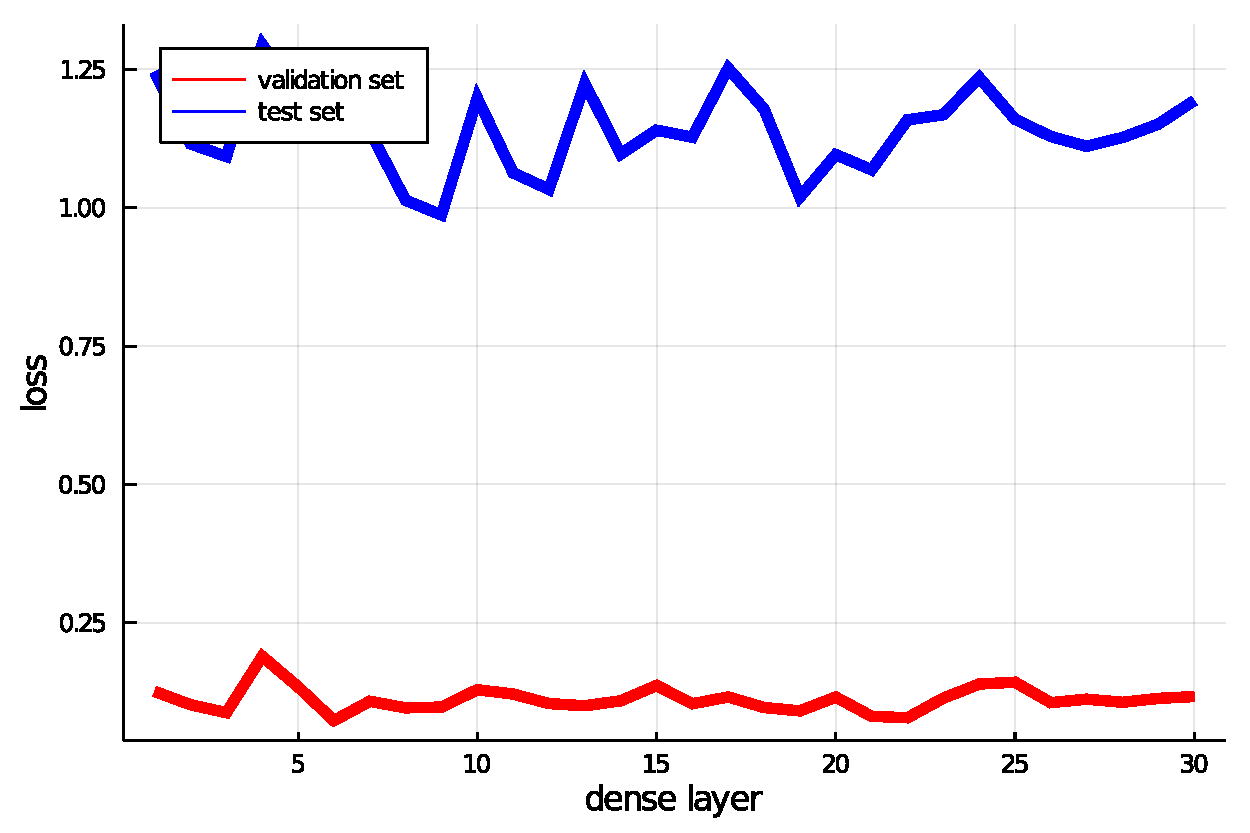
\includegraphics[width=8.0cm]{Images/TITLE/Newsgroups1} }}%
\
 \subfloat[]
{{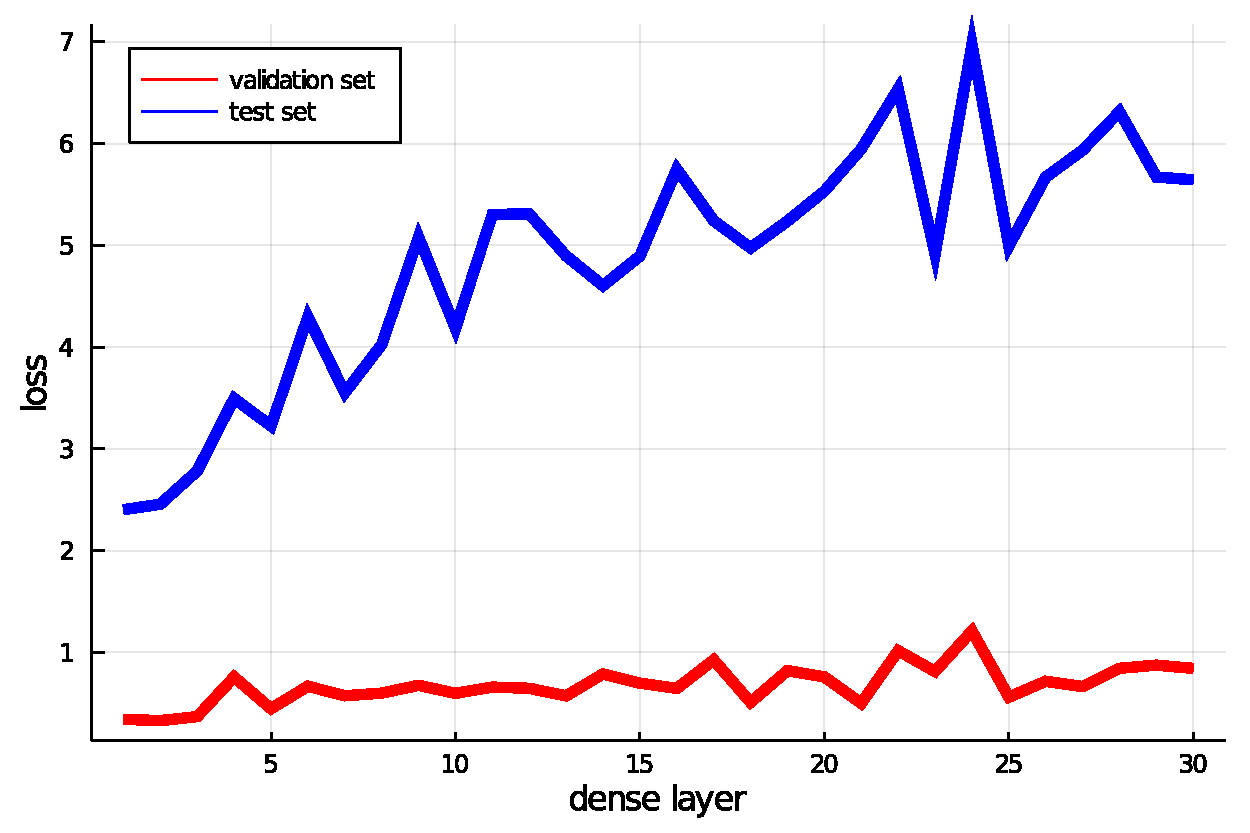
\includegraphics[width=8.0cm]{Images/TITLE/Musk1} }}%,
\subfloat[]
{{\includegraphics[width=8.0cm]{Images/TITLE/Newsgroups2} }}%
    \caption{Evaluation of loss function with the use of validation and test set on different MILL datasets.}%
    \label{CV}%
\end{figure}
As we can see in Figure \ref{CV}, the loss evaluated on different sets varies therefore it is likely to make mistakes when choosing our hyperparameter if we don't have enough input data.

\pagestyle{headings}

\section{Experiment with Point Cloud Mnist}
We applied previous method on Point Cloud Mnist 2D (PCM) dataset. However, we needed to make a little adjustment to this dataset, because we perform the binary classification. Originally, PCM has tottaly 10 labels (labels are numbers 0-9), so we separated arbitrarily 8 of them to obtain just 2 classes. In addition, we randomly split data into bags. \\
The advantage of PCM is that we can split the data into bags in many ways, e.g. 0\&1 , 2\&3, 5\&7,$\dots$ we can even take 0\&1 as first class and, for example, 2\&3 as a second class.
\begin{table}[h]
\centering
\begin{tabular}{|l|l|}
\hline
labels & difference \\ \hline
0\&1   & 0.81       \\ \hline
2\&3   & 2.07       \\ \hline
4\&5   & 2.05           \\ \hline
\end{tabular}
\end{table}
\begin{figure}[h]
\centering
\subfloat[]
{{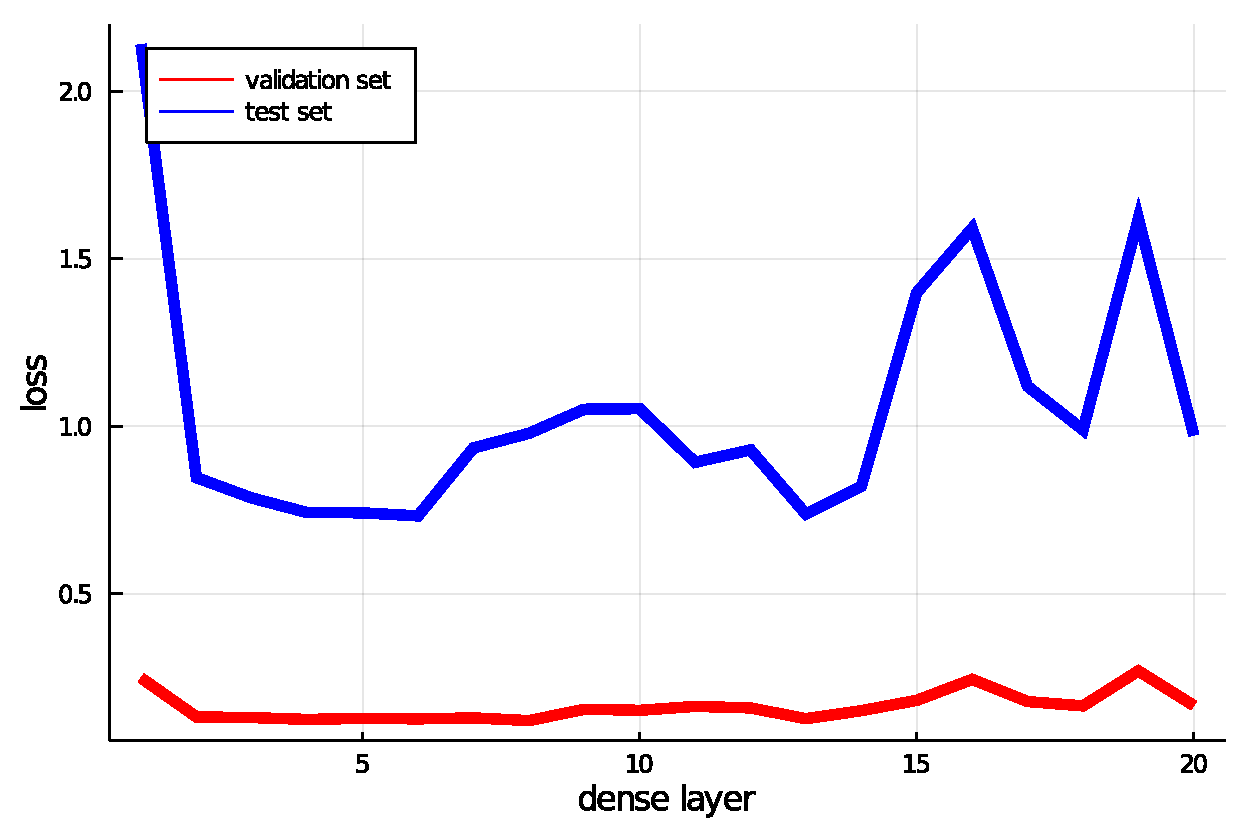
\includegraphics[width=8.0cm]{Images/TITLE/PCM01} }}%
\subfloat[]
{{\includegraphics[width=8.0cm]{Images/TITLE/PCM23} }}%
\
 \subfloat[]
{{\includegraphics[width=8.0cm]{Images/TITLE/PCM45} }}%,
 \caption{Evaluation of loss function with the use of validation and test set on Point Cloud Mnist}%
    \label{CVa}%
\end{figure}

\chapter*{Conclusion}

\pagestyle{plain}

\addcontentsline{toc}{chapter}{Conclusion}

Text of the conclusion\ldots{}
\begin{thebibliography}{1}
\bibitem{Allen-Cahn}S. Allen, J. W. Cahn: \emph{A microscopic theory
for antiphase boundary motion and its application to antiphase domain
coarsening}. Acta Metall., 27:1084-1095, 1979.

\bibitem{CINECA}G. Ballabio et al.: \emph{High Performance Systems
User Guide}. High Performance Systems Department, CINECA, Bologna,
2005. \url{www.cineca.it}

\bibitem{rumpf3}J. Becker, T. Preusser, M. Rumpf: \emph{PDE methods
in flow simulation post processing}. Computing and Visualization in
Science, 3(3):159-167, 2000.
\end{thebibliography}

\end{document}
